\section{Proof Production}
\label{sec:proofproduction}

In this section we describe how to produce resolution proofs from paths in a congruence graph.
The method to carry out this operation is \texttt{produceProof}.
The basic idea is to traverse the path, creating a transitivity chain of equalities between adjacent nodes, while keeping track of the deduced equalities in the chain.
From Invariant Deduced Edges follows that for the deduced equalities there have to be paths between the respective arguments of the compound terms.
These paths are transformed into proofs recursively and resolved with a suiting instance of the compatibility axiom.
After this operation the subproof is resolved with the original transitivity chain.
Since terms can never be equal to their (proper) subterms, the procedure will eventually terminate.
The result of this procedure is a resolution proof with a root, such that the equations of the negative literals are an explanation of the target equality or $\emptyset$ to denote that the equality can not be proven.
Suppose some equality $s \thickapprox t$ can be explained and \texttt{produceProof} returns a proof with root $\rho$, then it is the case that $neg(\rho) \models s \thickapprox t$ and $neg(\rho)$ is a subset of the input equations.

\begin{algorithm}[t]
\caption[.]{produceProof}
  \KwIn{term $s$}
	\KwIn{term $t$}
	%\KwIn{congruence graph $g$}
	\KwOut{Resolution proof for $E \models s \thickapprox t$ or $\emptyset$}
	
	$p \leftarrow explain(s,t,g)$ \\
	$d \leftarrow \emptyset$ \\
	$e \leftarrow \emptyset$ \\
	
	\While{$p$ is not empty}{
		$(u,l,v) \leftarrow $ first edge of $p$ \\
		$p \leftarrow p \setminus (u,l,v)$ \\
		$e \leftarrow e \cup \{u \neq v\}$ \\
		\If{$l = \smiley$}{
			$f(a,b) \leftarrow u$ \\
			$f(c,d) \leftarrow v$ \\
			$p_1 \leftarrow produceProof(a,c)$ \\
			$p_2 \leftarrow produceProof(b,d)$ \\
			$con \leftarrow \{ a \neq c, b\neq d, f(a,b) = f(c,d) \}$ \\
			$res \leftarrow$ resolve $con$ with non $\emptyset$ roots of $p_1$ and $p_2$ \\
			%$int_1 \leftarrow$ resolve $con$ with $root(p_1)$ \\
			%$int_2 \leftarrow$ resolve $int_1$ with $root(p_2)$ \\
			$d \leftarrow d \cup res$
		}
	}
	
	\If{$\# e > 1$}{
		$proof \leftarrow e \cup \{s = t\}$ \\
		\While{$d$ is not empty}{
			$int \leftarrow $ some element in $d$ \\
			$d \leftarrow d \setminus \{int\}$ \\
			$proof \leftarrow $ resolve $proof$ with $int$
		}
		\Return $proof$
	}
	\ElseIf{$d = \{ded\}$}{
		\Return $ded$
	}
	\Else{
		\If{$e = \{(u,l,u)\}$} {
			\Return $\{u = u\}$
		}
		\Else {
			\Return $\emptyset$
		}
	}
	
  \label{algo:prodproof}
\end{algorithm}



\begin{example}

Consider again the congruence graph shown in Figure \ref{fig:short_expl} and suppose we want a proof for $a \thickapprox b$.
Suppose we found the path $p_1 := \langle  a, f(c_1,e), f(c_4,e), c_1, c_2, c_3, c_4, b \rangle$ as an explanation and that the explanation for $f(c_1,e) \thickapprox f(c_4,e)$ is the path $\langle c_1, c_2, c_3, c_4 \rangle$.
We transform $p_1$ and $p_2$ into instances of the transitivity axiom $C_1$ and $C_2$ respectively. 
The clause $C_2$ is resolved with the instance of the congruence axiom $C_3$, which is then resolved with the instance of the reflexive axiom $C_4$ resulting in clause $C_5$.
Finally, $C_1$ is resolved with $C_5$ to obtain the final clause $C_6$.
The proof is shown in Figure \ref{fig:proofprod}.

\begin{figure}[!h]

\centering
\begin{tikzpicture}[node distance=1.5cm]
	%\proofnode{root} {$a \neq f(c_1,e), f(c_4,e) \neq c_1, c_1 \neq c_2, c_2 \neq c_3, c_3 \neq c_4, c_4 \neq b, a = b$};
	%
	%%\proofnode{root} {$C_6$};
	%
	%\withchildren{root} {c1}{$a \neq f(c_1,e), f(c_1,e) \neq f(c_4,e), f(c_4,e) \neq c_1, c_1 \neq c_2, c_2 \neq c_3, c_3 \neq c_4, c_4 \neq b, a = b$} {c5}{$c_1 \neq c_2, c_2 \neq c_3, c_3 \neq c_4, f(c_1,e) = f(c_4,e)$};
	%
	%\withchildren{c5} {c4}{$e = e$} {tmp}{tmp};
	%
	%\withchildren{tmp} {c3}{$e \neq e, c_1 \neq c_4, f(c_1,e) = f(c_4,e)$} {c2}{$c_1 \neq c_2, c_2 \neq c_3, c_3 \neq c_4, c_1 = c_4$};


	\proofnode[xshift=-1cm,font=\small,align=center]{root} {$C_6$\\$a \neq f(c_1,e), f(c_4,e) \neq c_1, c_1 \neq c_2, c_2 \neq c_3, c_3 \neq c_4, c_4 \neq b, a = b$};
	
	\proofnode[above left of=root,yshift=1.25cm,xshift=-2.75cm,align=center,font=\small]{c1}{$C_1$\\$a \neq f(c_1,e), f(c_1,e) \neq f(c_4,e), f(c_4,e) \neq c_1,$\\$ c_1 \neq c_2, c_2 \neq c_3, c_3 \neq c_4, c_4 \neq b, a = b$};
	\proofnode[above right of=root,yshift=.5cm,xshift=2cm,align=center,font=\small]{c5}{$C_5$\\$c_1 \neq c_2, c_2 \neq c_3, c_3 \neq c_4, f(c_1,e) = f(c_4,e)$};

	\proofnode[above left of=c5,xshift=-1.5cm,align=center,font=\small]{c4}{$C_4$\\$e = e$};
	\proofnode[above right of=c5,xshift=1cm,align=center,font=\small]{tmp}{$e \neq e, c_1 \neq c_2, c_2 \neq c_3, c_3 \neq c_4, f(c_1,e) = f(c_4,e)$};

	\proofnode[above left of=tmp,align=center,xshift=-2.5cm,font=\small]{c3}{$C_3$\\$e \neq e, c_1 \neq c_4, f(c_1,e) = f(c_4,e)$};
	\proofnode[above right of=tmp,align=center,yshift=1cm,xshift=-.75cm,font=\small]{c2}{$C_2$\\$c_1 \neq c_2, c_2 \neq c_3, c_3 \neq c_4, c_1 = c_4$};

	\drawchildren{root}{c1}{c5};
	\drawchildren{c5}{c4}{tmp};
	\drawchildren{tmp}{c3}{c2};
	
	%\proofnode[right of=root, xshift=2cm]{root2} {$t_a \neq a, a\neq b, b \neq t_b, t_a = t_b$};
	
\end{tikzpicture}


\caption{Example proof}
\label{fig:proofprod}
\end{figure}

\end{example}

As mentioned in Section \ref{sec:congruenceclosurealgorithm}, edges are inserted into a congruence graph in a lazy way by the congruence closure algorithm.
The reason is that \texttt{produceProof} searches for explanations for edges with label $\smiley$.
Should the equality of question be an input equation that is added later to the congruence structure than it was deduced, then we would like to overwrite this label with the input equation.
The impact of lazy insertion gets larger, if an implementation searches for explanations already when an edge is added to the graph.
Example \ref{example:lazy} shows how this technique can help producing shorter proofs.

\begin{example}
\label{example:lazy}
Suppose we want to add the following sequence of equations into an empty congruence structure: $\langle (a,b),(f(a,a),d),(f(b,b),e),(f(a,a),f(b,b)) \rangle$.
After adding the first three equations, the congruence closure algorithm detects the deduced equality $f(a,a) \thickapprox f(b,b)$.
The explanation for this equality is $\{(a,b)\}$, if we were to insert the edge $(f(a,a),f(b,b))$ into the graph immediately, it would have weight 1 and label $\smiley$.
Depending on the congruence graph used, when adding the fourth equation $(f(a,a),f(b,b))$ to the congruence structure, either the edge $(f(a,a),f(b,b))$ is not added at all to the graph or is added with weight 1.
In the latter case, both edges have weight 1 and equal chance to be selected by the shortest path algorithm.
However, choosing the edge with label $\smiley$ is undesirable, since it two extra resolution nodes (corresponding to the compatability axiom and an intermediate node).

\end{example}

\FloatBarrier

\subsection*{Congruence Compressor}

In this section we put our explanation producing congruence closure algorithm and the proof production method into the context of proof compression.
To this end we replace subproofs with conclusions that contain unnecessary long explanations with new proofs that have shorter conclusions.
Shorter conclusions lead to less resolution steps further down the proof and possibly large chunks of the proof can simply be discarded.
There is however a tradeoff in overall proof length when introducing new subproofs.
The subproof corresponding to a short explanation can be longer in proof length, i.e. involve more resolution nodes, than one with a longer explanation.
Example \ref{example:shortexpl} displays this issue.
Additionally it can be the case that by introducing a new subproof, we only partially remove the old subproof.
Some nodes of the old subproof might still be used in other parts of the proof.
Therefore the replacement of a subproof by another, smaller one does not necessarily lead to a smaller proof.
Nevertheless, our intuition is that favoring smaller conclusions should dominate such effects, especially on large proofs.

%In Section \ref{sec:proofprocessing} processing of a proof was defined.
%The most important application of proof processing for this work is proof compression.

\begin{example}
\label{example:shortexpl}
For presentation purposes, throughout this example we will abbreviate the term $f(f(a,b),f(a,a))$ with $t_a$ and $f(f(b,a),f(b,b))$ with $t_b$.
Consider the set of equations $E = \{(t_a,a),(a,b),(b,t_b)\}$ and the target equality $t_a \thickapprox t_b$.
Using equations in $E$, one can prove the the target equality in two ways.
Either one uses the instance of the transitivity axiom $\{t_a \neq a, a \neq b, b \neq t_b, t_a = t_b\}$ or a repeated applications of instances of the congruence axiom, e.g. $\{a \neq b, f(a,a) = f(b,b)\}$.
The corresponding explanations are $E$ and $\{(a,b)\}$.

The two resulting proofs are shown in Figure \ref{fig:short_expl_proof}.
The proof with the longer explanation $E$ is only one proof node, whereas the proof with the singleton explanation has proof length 5.

\begin{figure}[!h]

\centering
\begin{tikzpicture}[node distance=2.5cm]
	\proofnode[align=center]{root} {$a \neq b, t_a = t_b$\\Congruence proof};
	
	\proofnode[above left of=root,yshift=.25cm]{n5}{$a \neq b, f(a,a) \neq f(b,b), t_a = t_b$};
	\proofnode[above right of=root,yshift=-.25cm]{n7}{$a\neq b, f(a,a) = f(b,b)$};

	\proofnode[above left of=n5,yshift=.25cm]{n3}{$f(a,b) \neq f(b,a), f(a,a) \neq f(b,b), t_a = t_b$};
	\proofnode[above right of=n5,yshift=-.25cm]{n4}{$a \neq b, f(a,b) = f(b,a)$};

	\drawchildren{root}{n5}{n7};
	\drawchildren{n5}{n3}{n4};
	
	\proofnode[right of=root, xshift=2cm, align=center]{root2} {$t_a \neq a, a\neq b, b \neq t_b, t_a = t_b$\\Transitivity proof};
\end{tikzpicture}


\caption{Short explanation, long proof}
\label{fig:short_expl_proof}
\end{figure}

\end{example}

The Congruence Compressor compresses processes a proof replacing subproofs as described above. 
It is defined upon the processing function $f: V \times V \times V \rightarrow V$ specified in pseudocode in Algorithm \ref{algo:compressor}.
The function $g_f: V \rightarrow V$ for axioms is simply the identity (i.e. axioms are not modified).
The idea of the processing function is simple.
Axioms are not changed by the function.
For all other nodes the \texttt{fixNode} method is called, to maintain a correct proof.
For a clause $C$, the method adds $neg(C)$ (as defined in \ref{sec:calculus}) to the empty congruence structure and checks whether these equations induce a proof for one of the equations in the $pos(C)$ that has a shorter conclusion than the original subproof.
If there is such a proof, we replace the old subproof by the new one.
Example \ref{example:compressproof} displays this procedure.

In line \ref{criteria} it is decided whether the explanation finding congruence closure algorithm should be used to find a replacement for the current node.
A trivial criteria is true for every node.
Testing every node will result in a slow algorithm, but the best possible compression.
Some nodes do not need to be checked, since they contain optimal explanations by definition or there is no hope of finding an explanation at all.
The following definition classifies nodes to define a more sophisticated decision criteria.

\begin{definition}[Types of nodes]

An axiom is a \emph{theory lemma} if it is an instance of one of the congruence axioms.
Otherwise it is \emph{input derived}.
The classification of internal nodes is defined recursively.
An internal node is input derived, if one of its premises is input derived.
Otherwise it is a theory lemma.
We call a node a \emph{low theory lemma} if it is a theory lemma and has a child that is input derived.

\end{definition}

We suspect that most redundancies in proofs are to be found in low theory lemmas, since they reflect the explanations found by the proof producing solver.
Therefore an alternative criteria is to only find replacements for low theory lemmas.
The question whether a node is a low theory lemma is not trivial to answer while traversing the proof in a top to bottom fashion.
Therefore a preliminary traversal is necessary to determine the classification of nodes.
%Experiments have shown that using this criteria speeds up the algorithm a lot, while losing only very little compression.
Further criteria for deciding whether or not to replace could be size of the subproof or a global metric that tries to predict the global compression achieved by replacement.

\begin{algorithm}[h]
\caption[.]{compress}
	\KwGlobal{set of input equations $E$}
	\KwIn{resolution node $n$}
  \KwIn{$pr:$ tuple of resolution nodes $(p_1,p_2)$}
	\KwOut{resolution node}

	$m \leftarrow fixNode(n,(p_1,p_2))$ \\
	\If{$m$ fulfills criteria \label{criteria}}{
		$lE \leftarrow \{(a,b) \mid (a \neq b) \in m\}$ \\
		$rE \leftarrow \{(a,b) \mid (a = b) \in m\}$ \\
		$con \leftarrow $ empty congruence structure \\
		\For{$(a,b)$ in $lE$}{
			$con \leftarrow con.addEquality(a,b)$
		}
		\For{$(a,b)$ in $rE$}{
			$con \leftarrow con.addNode(a).addNode(b)$ \\
			$proof \leftarrow con.prodProof(s,t)$ \\
			\If{$proof \neq \emptyset$ and $| proof.conclusion | < | m.conclusion |$}{
				$m \leftarrow proof$
			}
		}
	}
	\Return $m$
  \label{algo:compressor}
\end{algorithm}


The compressor (Algorithm \ref{algo:compressor}) uses the method \texttt{fixNode} to maintain a correct proof.
The method modifies nodes with premises that have earlier been replaced by the compressor. 
Nodes with unchanged premises are not changed.
Let $n$ be a proof node that was derived using pivot $\ell$ in the original proof and which updated premises are $pr_1$ and $pr_2$ .
Depending on the presence of $\ell$ in $pr_1$ and $pr_2$, $n$ is either replaced by the resolvent of $pr_1$ and $pr_2$ or by one of the updated premises.
In case both updated premises do not contain the original pivot element, replacing the node by either one of them maintains a correct proof.
Since we are interested in short proofs, we return the one with the shorter clause.
This method of maintaining a correct proof was proposed in \cite{Bar-Ilan2008} in the context of similar proof compression algorithms.

\begin{algorithm}[h]
\caption[.]{fixNode}
	\KwIn{resolution node $n$}
  \KwIn{$pr:$ tuple of resolution nodes $(p_1,p_2)$}
	\KwOut{resolution node}
	
	\eIf{($n.premise_1 = p_1$ and $n.premise_2 = p_2$)}{
		\Return $n$
	}{
		\If{$n.pivot \in p_1$ and $n.pivot \in p_2$}{
			\Return $resolve(p_1,p_2)$
		}
		\ElseIf{$n.pivot \in p_1$}{
			\Return $p_2$
		}
		\ElseIf{$n.pivot \in p_2$}{
			\Return $p_1$
		}
		\Else{
			\Return node with smaller clause
		}
	}

  \label{algo:fixnode}
\end{algorithm}



\begin{example}
\label{example:compressproof}
Consider the proof presented graphically in Figure \ref{fig:compressproof}.
It uses the same abbreviations for $t_a$ and $t_b$ as in Example \ref{example:shortexpl}.
Furthermore, the proof uses the long explanation for $t_a \thickapprox t_b$.
The length of the proof is 12.
The proof contains one propositional variable $A$.
The compression algorithm traverses the proofs and detects the redundant explanation in node $O_1$.
The subproof $N_1$ corresponding to the explanation $\{(a,b)\}$ is created and $O_1$ is replaced by it.
The construction of this subproof is discussed in Example \ref{example:shortexpl}.
When iterating over node $O_2$, the algorithm detects that the pivot literal $t_a = a$ is not present in $N_1$ and \texttt{fixNode} replaces $O_2$ by $N_1$.
At node $O_3$, both premises contain the pivot $a = b$, therefore $O_3$ is replaced by resolvent of $N_1$ and its other original premise.
No other subproof is altered by the algorithm.
The resulting proof is displayed in Figure \ref{fig:compressproof_2} and has length 11 which is shorter than the original one, even though the replaced subproof is larger.
Note that the clause $\{\neg A\}$ is part of the replaced subproof.
It is also part of the subproof with conclusion $\{a = b\}$, which remains in the new proof.

\begin{figure}[!h]

\centering
\begin{tikzpicture}[node distance=2.5cm]

	\rootnode;
	
	\withchildren{root}{n11}{$t_a = t_b$} {n10}{$t_a \neq t_b$};

	\proofnode[above left of=n11, align=center,font=\small]{n9}{$b \neq t_b$};
	\proofnode[above right of=n11, align=center,font=\small]{n8}{$O_3$\\$b \neq t_b, t_a = t_b$};
	\drawchildren{n11}{n9}{n8};
	\proofnode[above left of=n8, align=center,font=\small]{n5}{$O_2$\\$a \neq b, b\neq t_b, t_a = t_b$};
	
	\proofnode[above left of=n5, align=center,font=\small]{n1}{$O_1$\\$t_a \neq a, a\neq b, b \neq t_b, t_a = t_b$};
	\proofnode[above right of=n5]{n4}{$t_a = a$};
	\drawchildren{n5}{n1}{n4};
	\proofnode[above left of=n4]{n2}{$A,t_a = a$};
	
	
	
	\proofnode[right of =n4]{n7}{$a = b$};
	\drawchildren{n8}{n5}{n7};
	\withchildren{n7}{n3}{$\neg A$} {n6}{$A, a = b$};
	\drawchildren{n4}{n2}{n3};
\end{tikzpicture}


\caption{Original Proof}
\label{fig:compressproof}
\end{figure}

\begin{figure}[!h]

\centering
\begin{tikzpicture}[node distance=2.5cm]
	
	
	\rootnode;
	
	\withchildren{root}{new9}{$t_a = t_b$} {new10}{$t_a \neq t_b$};
	
	\proofnode[above right of=new9,yshift=-1cm,xshift=.5cm]{new8}{$a = b$};

	\proofnode[above left of=new9, align=center,font=\small]{new5} {$N_1$\\$a \neq b, t_a = t_b$};
	
	\proofnode[above left of=new5,yshift=.25cm]{n5}{$a \neq b, f(a,a) \neq f(b,b), t_a = t_b$};
	\proofnode[above right of=new5,yshift=-.25cm]{n7}{$a\neq b, f(a,a) = f(b,b)$};

	\proofnode[above left of=n5,yshift=.25cm]{n3}{$f(a,b) \neq f(b,a), f(a,a) \neq f(b,b), t_a = t_b$};
	\proofnode[above right of=n5,yshift=-.25cm]{n4}{$a \neq b, f(a,b) = f(b,a)$};

	\drawchildren{new5}{n5}{n7};
	\drawchildren{n5}{n3}{n4};
	
	\drawchildren{new9}{new5}{new8};
	
	\withchildren{new8}{new6}{$\neg A$} {new7}{$A,a = b$};
\end{tikzpicture}


\caption{Compressed Proof}
\label{fig:compressproof_2}
\end{figure}

\end{example}

\FloatBarrier
